
\chapter{人机交互式机器翻译方法综述}
\label{Chapter_overview}

\section{概述}

虽然利用机器翻译提高人工翻译效率的想法早已有之,但由于早期机器翻译系统的翻译质量距离能辅助专业译员的程度有很大差距,并且机器翻译与计算机辅助翻译的应用场景也有所不同,因此二者各自独立发展了很多年。机器翻译与计算机辅助翻译的核心议题是翻译自动化,即机器在翻译中的比重。前者主要强调翻译的主体是机器,而后者强调人工为主、机器为辅的翻译。

直到最近几年,随着统计机器翻译和神经网络机器翻译质量的不断提高,研究人员才开始关注如何进一步改善专门面向计算机辅助翻译的机器翻译,在后文中我们称之为人机交互式机器翻译。

从发展时间来看,计算机辅助翻译是机器翻译的译文质量过低的产物。机器翻译兴起于20世纪50年代初,20世纪90年代以前,机器翻译的主流方法是基于规则的方法。由于当时的自动译文质量过低,最先被提出的译后编辑也得不到广泛应用。完全不用机器翻译的计算机辅助翻译起步于20世纪80年代,核心是翻译记忆。直到2002年,语料库技术和统计学习方法在机器翻译中得到广泛应用之后,交互式机器翻译方法才被提出。但时至今日,交互式机器翻译方法也未得到实际应用。在本文中,我们将文献[\cite{Foster:2002,Koehn:2014}]中介绍的根据用户输入前缀重新解码的交互式机器翻译作为 “人机交互式机器翻译”的一种具体表现形式。在后文中,如无特别说明,“人机交互式机器翻译”指范围更广的面向计算机辅助翻译的机器翻译。

本章先给出统计机器翻译和神经网络机器翻译的问题定义,并简要介绍机器翻译发展至今所出现的主要模型。再给出计算机辅助翻译问题的定义,并详细介绍人机交互式机器翻译方法及在人工翻译场景中存在的问题,引出本文将要开展的创新性研究。


\section{机器翻译}

20世纪90年代以前,机器翻译的主流方法是基于规则的方法,即利用语言学家设计的转换规则进行翻译。这通常需要源语言和目标语言的词汇、句法以及语义知识。优点是能较好地保持原文的结构,对于规则所覆盖的语言现象翻译较好。缺点是规则需要由专业人员撰写和维护,因此工作量大,主观性强,一致性难以保障,不利于系统的扩充。这些都制约着基于规则的方法的发展和应用。

20世纪90年代初,语料库技术和统计学习方法在机器翻译中得到广泛的应用。机器翻译因而进入蓬勃发展期,打破了长期以来分析方法占主导地位的局面。基于语料库的机器翻译方法,可以分为四类:(1)基于记忆的翻译方法(memory-based machine translation);(2)基于实例的机器翻译方法(example-based machine translation,EBMT)[\cite{Nagao:1984}];(3)基于统计的机器翻译方法(statistical machine translation,SMT)[\cite{Brown:1990,Brown:1993,Koehn:2003,Koehn:2007,Chiang:2005,Chiang:2007}];(4)基于神经网络的机器翻译方法(neural machine translation, NMT)。

基于记忆的翻译方法假设人类进行翻译时是根据以往的翻译经验进行的,不需要对句子进行语言学上的深层分析,翻译时只需要将句子拆分成适当的片断,然后将每一个片断与已知的例子进行类比,找到最相似的句子或片断所对应的目标语言句子或片断作为翻译结果,最后将这些目标语言片断组合成一个完整的句子[\cite{Sato:1990}]。

\begin{figure}[!htbp]
	\centering
	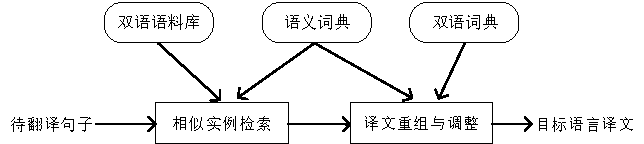
\includegraphics[width=0.9\textwidth]{Figure/Figure_2_1.pdf}
	\caption{基于实例的机器翻译方法基本结构图}
	\label{Fig_ebmt}
\end{figure}

基于实例的方法一般如图\ref{Fig_ebmt}所示部分构成,首先需要对已知语料进行词法、句法,甚至语义等分析,建立实例库用以存储翻译实例。系统在执行翻译过程时,查找与待翻译句子最相似的翻译实例,最后根据找到的相似实例的译文得到翻译句子的译文。因此基于实例的方法对于相似的文本效果很好,但它受限于实例库的规模。此外,与统计机器翻译方法相比,它并没有严谨的数学模型可对系统进行优化。因此近年来已逐步淡出舞台。

基于统计的翻译方法,则主张对翻译过程先进行数学建模,再通过大规模双语平行语料库来估计模型参数,然后利用估计好的模型进行翻译。与基于规则的翻译方法相比,统计机器翻译只需要双语平行语料,就可以自动地学习翻译知识。与基于实例的翻译方法相比,统计机器翻译有严谨的数学模型,及对系统进行优化的理论基础,因而可以获得更好的结果,所以成为机器翻译技术的主流之一。然而,由于统计机器翻译方法采用离散符号来表示翻译知识,导致它还存在一些难以回避的问题,如长句和复杂句式的处理问题,弱规范甚至非规范化文本的翻译问题,增长式学习问题和反馈学习问题。

最近几年,深度学习在语音识别和图像处理领域取得了突破性进展。深度学习擅长于无监督的特征学习,能够学到高度抽象的语义表示。而目前的统计机器翻译使用的都是人工设计的特征。于是研究人员开始尝试使用神经网络中的连续向量表示来对翻译过程进行建模。经过短短两三年的发展,该方法就达到了与传统统计机器翻译方法相媲美的效果[\cite{Kalchbrenner:2013,Sutskever:2014,Cho:2014,Bahdanau:2015}]。所以这两年神经网络方法成为机器翻译方法的主流之一,且热度一度超过了统计机器翻译。需要指出的是,神经网络机器翻译也面临着很多新的问题和挑战,需要人们进行更加深入的研究,如重复翻译与漏翻译,词对齐效果不理想,流畅性好而忠实度差,难以融合命名实体和术语翻译知识等问题。

\subsection{统计机器翻译}

\begin{figure}[!htbp]
	\centering
	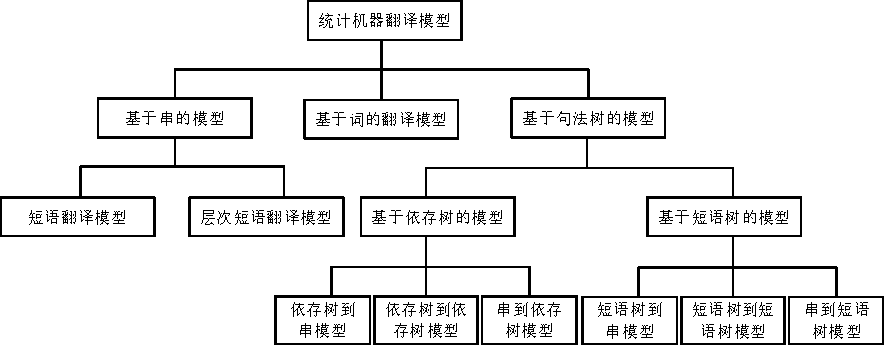
\includegraphics[width=0.9\textwidth]{Figure/Figure_2_2.pdf}
	\caption{统计机器翻译的典型翻译模型}
	\label{Fig_smt_model}
\end{figure}

统计机器翻译的基本思想是充分利用机器学习技术从大规模双语平行语料中自动获取翻译规则及其概率参数,然后利用翻译规则对源语言句子进行解码。对于给定的源语言句子$s$,统计机器翻译认为其翻译可以是任意的目标语言句子$t$,只是不同目标语言句子的概率不同。而统计机器翻译的任务,就是从所有的目标语言句子中,找到概率最大的译文$\widehat{t}$:

\begin{equation}
\label{Eq_smt_argmax}
\widehat{t} = \mathop{\argmax}_{t}{P(t|s)}
\end{equation}

虽然自然语言的词汇量是有限的,但其组成的句子数量却是无限的。因此,公式\ref{Eq_smt_argmax}仅仅给出了一个形式化的定义,直接估计概率 是不可行的。我们需要对整个翻译过程进行分解和建模,将概率 转换为若干个概率的乘积,并将统计机器翻译问题转化为分别估计这些概率。这个过程即用数学模型描述从源语言到目标语言的转换过程。最终所建立的模型为翻译模型(translation model),即在给定源语言句子的条件下,确立不同译文的翻译概率的计算方法。研究者们使用大规模的双语语料来学习翻译模型的参数,这个过程被称为训练(training)。最后,利用翻译模型和训练得到的概率,根据公式\ref{Eq_smt_argmax}寻找最优的翻译结果,这一过程被称为解码(decoding)。

在上面三个过程中,翻译模型是统计机器翻译研究的基础和核心,它直接决定了参数估计和解码算法的设计。训练和解码都建立在翻译模型的基础之上。图\ref{Fig_smt_model}给出了当前统计机器翻译的一些典型翻译模型[\cite{zhangzong:2013}]。接下来我们回顾统计机器翻译的发展历程,并阐述我们为什么要选择基于短语的翻译模型作为基线系统。

\textbf{(1)基于词的翻译模型}

基于词的翻译模型是最简单的统计机器翻译模型,里程碑事件是由IBM的研究人员Brown等人[\cite{Brown:1990,Brown:1993}]提出了著名的IBM模型1到模型5。IBM模型1到模型5都是基于噪声信道模型,根据贝叶斯模型,公式\ref{Eq_smt_argmax}可以转化为:

\begin{equation}
\label{Eq_smt_argmax_detail}
\begin{split}
\widehat{t} & = \mathop{\argmax}_{t}{P(t|s)} \\
& = \mathop{\argmax}_{t}{\frac{P(s|t) \times P(t)}{P(s)}} \\
& = \mathop{\argmax}_{t}{P(s|t) \times P(t)} 
\end{split}
\end{equation}

其中,$P(t)$为用来控制译文流畅性的语言模型,$P(s|t)$为用来控制译文对源语言句子忠实度的翻译模型。IBM模型1到模型5都是以词作为基本翻译单位,不同词汇的翻译是孤立的,需要一个双语词典将两种语言中互为翻译的词汇关联起来。这5个模型的复杂度依次递增。虽然这一技术已经跟不上最新的技术水平,但奠定了统计机器翻译的理论基础,其中的许多原则和方法现在依然适用。

研究人员在IBM模型的基础上,做了许多改进工作,其中比较有代表性的工作是Vogel等人提出了基于隐马尔科夫的词对齐模型[\cite{Vogel:1996}]。另外一个具有重大意义的工作是Och等人开发和优化了词对齐工具包GIZA++。GIZA++不仅实现了基于IBM模型1到模型5以及基于隐马尔科夫的词对齐模型,还提出了更为复杂的模型6[\cite{Och:2003b}]。

虽然基于词的翻译模型的数学描述十分完备,但也无法避免如下明显的缺点:以词作为基本单位,缺乏上下文信息;局部和全局调序能力都比较弱。虽然以后不再直接使用IBM模型,但它是其它统计机器翻译模型的基础。GIZA++更是成为统计机器翻译中的重要工具之一。

\textbf{(2)基于短语的翻译模型}

为了解决基于词的翻译模型中存在的问题和缺陷,研究人员开始探索基于短语的翻译模型[\cite{Wang:1998,Och:1999,Och:2002,Koehn:2003,Koehn:2004a,Koehn:2007}]。这里的“短语”表示任何连续的词串,区别于语言学上的“短语”。

基于短语的翻译模型(phrase-based translation model)是统计机器翻译之中最为成熟的模型。该模型的基本思想是:首先从双语句子对齐的平行语料库中抽取短语到短语的翻译规则,在翻译时将源语言句子切分为短语序列,利用翻译规则得到目标语言的短语序列,然后借助调序模型对目标语言短语序列进行排序,最终获得最佳的目标译文。短语翻译模型的翻译过程如图2.3(a)所示。

基于短语的翻译模型的一个重要工作是Och等人在最大熵(maximum entropy,ME)模型[\cite{Berger:1996}]的基础上,首次将对数线性模型引入到统计机器翻译中[\cite{Och:2002}]。他们发现,公式\ref{Eq_smt_argmax_detail}中的$P(s|t)$被其逆向翻译概率$P(t|s)$代替后,也能取得相似的翻译性能。因此可以直接对翻译的后验概率$P(t|s)$进行建模,即,对于给定的待翻译源语言句子$s$,它的最佳译文$t$可以表示为:

\begin{equation}
\label{Eq_smt_argmax_further}
\begin{split}
\widehat{t} & = \mathop{\argmax}_{t}{P(t|s)} \\
& = \mathop{\argmax}_{t}{\frac{\exp \sum_{m=1}^M \lambda_mh_m(s,t)}{\sum_{t'} \exp \sum_{m=1}^M \lambda_mh_m(s,t')}} \\
& = \mathop{\argmax}_{t}{ \left[ \exp \sum_{m=1}^M \lambda_mh_m(s,t) \right] } 
\end{split}
\end{equation}

其中,$h_m(s,t)$是翻译模型的特征函数,包括语言模型、翻译模型和调序模型等,而$\lambda_m$是这些特征函数对应的权重。针对对数线性模型,Och提出了最小错误率训练(minimum error rate training,MERT)方法。该方法根据线性模型的特点,使用直线的交点作为临界点,大大提升了训练速度。目前,最小错误率训练被广泛用作对数线性模型的参数训练方法。

由公式\ref{Eq_smt_argmax_further}可以知道,对数线性模型的引入使机器翻译系统不再仅仅依赖于翻译模型和语言模型,而是可以有效地利用多种有益信息,其中就包括非常重要的调序模型。与基于词的翻译模型相比,基于短语的翻译模型能够更好地捕捉局部上下文信息,同时还在短语内部隐含了局部调序信息,取得了更好的翻译质量。然而,由于基于短语的模型没有整合长距离的调序信息。因此,通过调序模型进行短语之间的调序操作一直是它的弱点。同时,调序模型也是统计机器翻译研究的重点和难点。当前主流的短语调序模型包括基于距离的短语调序模型、词汇化的短语调序模型和句法指导的短语调序模型[\cite{zhangjiajun:2011}]。

基于距离的短语调序模型类似于基于词的调序模型,根据跳转长度对短语调序进行建模。在此基础上,Zens等人利用IBM模型和反向转录文法[\cite{Wu:1997}]约束对调序空间进行限制[\cite{Zens:2003}]。但基于距离的调序模型太过简单,仅以短语移动的距离为条件,调序效果并不理想。
词汇化的短语调序模型以当前翻译的短语为条件,判断接下来翻译的短语与它的位置关系,如此更能把握实际语言中不同短语的调序特点[\cite{Tillmann:2004,Kumar:2005}]。实验表明词汇化的调序模型显著地改善了翻译质量。
句法指导的短语调序模型研究的重点是如何将句法知识有效地融入到调序模型中。文献[\cite{Collins:2005,Wang:2007,LiChiho:2007}]利用句法知识对源语言句子进行预调序,使之更接近目标语言句子的结构,然后利用通用翻译系统进行翻译。而文献[\cite{Zhang:2007,Xiong:2008,Zhang:2009,Zhang:2013}]则是把基于句法约束的调序模型融合到解码器中。两类模型都取得了不错的翻译效果,说明句法知识能够有效地帮助解码器获得更好的调序质量。
基于短语的翻译模型发展至今已经取得了很好的翻译质量和性能。基于短语的翻译模型的一个重要标志性工作是Koehn等人开发的开源解码器Moses[\cite{Koehn:2007}]。但是由于建模过程中所使用的知识十分有限,基于短语的模型也有其明显的缺点,即难以有效地处理长距离调序和非连续短语的问题。因此,研究者开始探索更为高级的翻译模型,基于句法的翻译模型随之产生。

\textbf{(3)基于句法的翻译模型}

根据引入句法信息的不同,基于句法的翻译模型可以分为两类:基于形式化句法的翻译模型和基于语言学句法的翻译模型。前者建立在形式化语法的基础之上,不包含任何语言学句法信息。后者主要建立在语言学语法基础上,利用语言学句法结构来指导翻译过程。由于本文不采用基于句法的翻译模型,下面我们将简略介绍部分相关工作。

\textbf{(3.1)基于形式化句法的翻译模型}

\begin{figure}[tb]
	\centering
	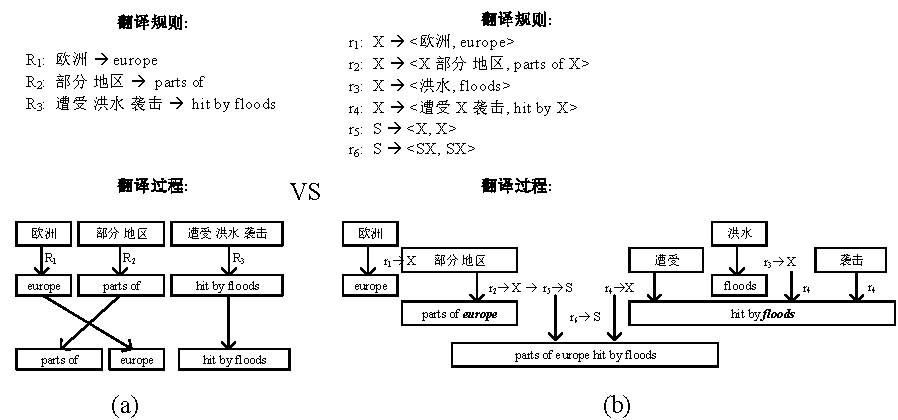
\includegraphics[width=0.9\textwidth]{Figure/Figure_2_3.pdf}
	\caption{短语翻译模型(a)与层次短语翻译模型(b)}
	\label{Fig_smt_phrase_hier}
\end{figure}

形式化语法主要以同步上下文无关文法(synchros context free grammar, SCFG)为代表,最初是用于双语同步分析。基于形式化句法的翻译模型,旨在借助形式化语法的结构,实现层次化的翻译过程。尽管这种层次化并不符合语言学意义上的句法概率,但可以在一定程度上处理长距离调序。

两个有代表的基于形式化句法的翻译模型是:(1)反向转录文法(inversion transduction grammar,ITG)模型[\cite{Wu:1997}];(2)层次短语模型(Hierarchical phrase=based model)[\cite{Chiang:2005,Chiang:2007}]。

其中层次短语模型,是统计机器翻译发展过程中的一个突破性工作。图\ref{Fig_smt_phrase_hier}以汉英翻译为例对比了短语翻译模型与层次短语翻译模型。由图\ref{Fig_smt_phrase_hier},我们可以看出,若翻译规则中的短语含有变量,短语翻译模型就发展成为基于层次短语的翻译模型,具有更强的表达能力,能够取得更好的翻译性能。短语模型翻译过程中需要短语调序模型的参与,而在层次短语模型中短语调序隐含于翻译规则当中。

\textbf{(3.2)基于语言学句法的翻译模型}

根据引入语言学句法的不同,基于语言学句法的翻译模型可以分为:(1)以依存结构树来指导翻译过程的基于依存语法的翻译模型;(2)以短语结构树来指导翻译过程的基于短语结构语法的翻译模型。从目前已取得的效果来看,基于短语结构语法的翻译模型要比基于依存语法的翻译模型更为成熟。

\begin{figure}[tb]
	\centering
	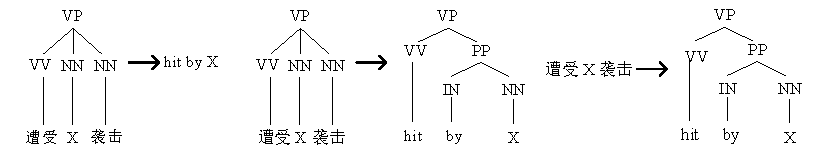
\includegraphics[width=0.95\textwidth]{Figure/Figure_2_4.pdf}
	\caption{基于语言学句法的翻译模型}
	\label{Fig_smt_syntax}
\end{figure}

根据翻译过程中语言学句法知识作用范围的不同,基于语言学句法的翻译模型又可以分为:

\begin{itemize}
	\item 串到树(string-to-tree):源语言端的字符串转换成目标语言端的句法树,仅利用目标语言端的句法树[\cite{Yamada:2001,Yamada:2002,Galley:2004,Marcu:2006,Shen:2008}],如图\ref{Fig_smt_syntax}(c)示。
	
	\item 树到串(tree-to-string):源语言端的句法树转换成目标语言端的字符串。仅使用源语言端的句法树[\cite{Huang:2006,LiuYang:2006,LiuYang:2007,Mi:2008,liuyangphd:2007,mihaitao:2009}],如图\ref{Fig_smt_syntax}(a)所示。
	
	\item 树到树(tree-to-tree):源语言端的句法树转换成目标语言端的句法树。同时使用源语言端和目标语言端的句法树[\cite{Zhang:2008b,LiuYang:2009,Chiang:2010}],如图\ref{Fig_smt_syntax}(b)所示。
\end{itemize}

串到树模型和树到串模型是基于句法的翻译模型中最成功的,目前还没有特别成功的树到树模型[\cite{zhangjiajun:2011}]。

\textbf{(4)基于语义的翻译模型}

句法结构的引入大大改善了翻译质量,但句法结构仅仅表示了句法层面的信息,而并没有表示句子内部不同成分之间的语义关系。因此,研究人员一直希望能将语义信息引入机器翻译模型中。基于语义的翻译模型又可分为如下两种:

\begin{itemize}
	\item 用词义消歧(word sense disambiguation,WSD)辅助机器翻译:如文献[\cite{Carpuat:2005}]提出的方法,首先对源语言中的每个实词进行词义消歧确定每个词紧随可能的义项,然后利用知网(Hownet)确定这个记号紧随可能的翻译。另一种方法是定位于翻译规则的消歧[\cite{Carpuat:2007,Chan:2007}]。
	
	\item 用谓词论元结构(predicate-argument structure,PAS)辅助机器翻译:文献[\cite{Fung:2006,Fung:2007,Wu:2009}]研究了谓词论元结构的双语特性,并确定谓词论元结构在翻译过程中比句法结构的一致性要强,因此它在理论上更适合于机器翻译。研究者提出了各种各样的方法来将谓词论元结构用于翻译,例如预处理和后处理[\cite{Komachi:2006,Wu:2011,Wu:2009}]、利用语义角色完善非终结符[\cite{LiuGildea:2010,Aziz:2011,Gao:2011}]、作为相关特征融入现有系统[\cite{LiuGildea:2010,Xiong:2012}]等。
\end{itemize}

总的来说,基于词的翻译模型已经退出了历史舞台,目前统计机器翻译的主流方法是基于短语的翻译模型和基于句法的翻译模型。同基于句法的翻译模型相比,基于短语的模型的翻译性能与其相当,但速度更快更稳定,而且与语言完全无关。正由于以上优点,基于短语的翻译模型仍然是目前的主流统计机器翻译模型。在本文工作中,我们也使用基于短语的翻译模型作为基线系统。

\begin{figure}[tb]
	\centering
	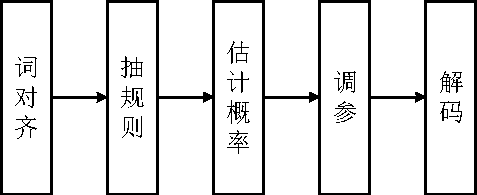
\includegraphics[width=0.6\textwidth]{Figure/Figure_2_5.pdf}
	\caption{统计机器翻译模块}
	\label{Fig_smt_modual}
\end{figure}

统计机器翻译的训练需要依次进行双语词对齐、抽取翻译规则、估计翻译概率以及在开发集上调节特征权重等步骤,如图\ref{Fig_smt_modual}所示。在统计机器翻译的训练过程中,每一步产生的错误都会影响到后续环节。尽管统计机器翻译中也有一些工作尝试融合其中的某些模块,例如跳过词对齐直接推导短语级别的对应关系[\cite{Cherry:2007,DeNero:2008,Zhang:2008c,Blunsom:2009,Neubig:2011,Levenberg:2012}],或者直接在训练集上学习每条翻译规则的权重[\cite{Liang:2006,Yu:2013}],但是这些方法都大大地增加了训练的复杂度,并且也没有取得非常理想的效果。

\subsection{神经网络机器翻译}

神经网络机器翻译(neural machine translation,NMT)是近年来兴起的一种全新的机器翻译方法,其基本思想是使用神经网络直接将源语言文本映射为目标语言文本。完全不同于传统机器翻译中以基于离散符号的转换规则为核心的做法,神经网络机器翻译使用连续的向量表示对翻译过程进行建模,因而能从根本上克服传统机器翻译中的泛化性能不佳、独立性假设过强等问题。

神经网络在机器翻译中的早期应用是作为特征融入到已有模型中[\cite{Yang:2013,Zou:2013,LiPeng:2013,Vaswani:2013,Tamura:2014,Gao:2014,Zhang:2014a,Zhang:2014b,Cui:2014,LiPeng:2014,Devlin:2014}],用以增强原有的词对齐、语言模型、调序模型和翻译模型等模块,取得了非常显著的效果。完全使用神经网络进行端到端的机器翻译的方法最早由[Kalchbrenner and Blunsom, 2013]提出。他们使用了编码器—解码器(encoder-coder)这一全新框架来描述翻译过程:给定一个源语言句子,首先使用一个编码器将其映射为一个连续的向量,然后再使用一个解码器根据该向量逐词生成目标语言句子。他们在论文中使用的编码器是卷积神经网络, 而解码器是循环神经网络。尽管该方法没有获得理想的翻译性能,但它开创了使用神经网络进行端到端机器翻译的先河,后续神经网络机器翻译的研究均沿用了编码器-解码器这一框架。

\begin{figure}[tb]
	\centering
	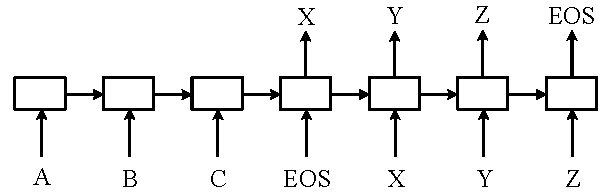
\includegraphics[width=0.8\textwidth]{Figure/Figure_2_6.pdf}
	\caption{神经网络机器翻译示意图}
	\label{Fig_nmt}
\end{figure}

Google 公司的 Ilya Sutskever 等人[\cite{Sutskever:2014}]使用循环神经网络同时作为编码器和解码器,并且他们采用了长短期记忆网络(Long Short Term Memory)[H\cite{Hochreiter:1997}]来取代原始的循环神经网络,以解决训练过程中的“梯度弥散”和“梯度爆炸”问题。他们的模型架构如图 2.6所示。给定一个源语言句子“A B C”,该模型逐个读入源语言单词并生成隐含向量表示,用以概括从句首到当前位置的所有信息,直到读入句子结束符“EOS”完成编码过程。解码时,模型根据历史信息生成每一时刻的隐含向量表示,并根据向量表示预测出目标语言单词“X Y Z”,直到生成“EOS” 结束。由于长短期记忆网络的引入,该模型取得了与传统的统计机器翻译相当的效果。

神经网络机器翻译的另一标志性工作来自蒙特利尔大学的 Bengio 等人[\cite{Bahdanau:2015}]。他们在编码器-解码器的基础上增加了注意力(attention)模型。受到认知科学中注意力机制的启发,作者认为解码器在生成每个目标语言单词时,只有少量源语言单词是高度相关的。为了达到这个效果,他们提出在预测每个目标语言单词时,使用动态的源端表示以突出相关信息,而不是对所有单词都采用固定的源端表示。他们的实验表明,注意力模型能更好地处理长距离依赖,显著提升神经网络机器翻译的质量。

神经网络机器翻译与传统的统计机器翻译相比,最本质的区别在于,前者采用的是离散符号到连续向量再到离散符号的转换,而后是离散符号到离散符号的转换。因此,神经网络机器翻译具有更好的泛化性。另外,神经网络机器翻译在建模时不使用任何独立性假设,它在预测每一个目标端单词时能使用所有的历史信息。更重要的是,神经网络机器翻译不需要人为地设计特征,这将机器翻译任务的自动化程度又向前推进了一步。当然,新的神经网络机器翻译也面临着很多新的问题和挑战,需要人们进行更加深入的研究,如重复翻译与漏翻译,词对齐效果不理想,流畅性好而忠实度差的问题,人工难以干预译文输出等。由于本文不采用神经网络机器翻译,因此这里不再赘述。

\section{计算机辅助翻译}

由于机器翻译存在语种或领域受限、记忆库或术语库无法挂接、自动译文难以干预等问题,目前尚无一款机器翻译系统能在无人工干预状态下满足用户所有翻译需求,因此计算机辅助翻译依然是人工翻译的主流工具。计算机辅助翻译帮助专业译员优质、高效、轻松地完成翻译工作。不同于机器翻译,计算机辅助翻译不依赖于机器翻译,而是在人的参与下完成整个翻译过程。但借助翻译流程自动化,与相同质量的人工翻译相比,计算机辅助翻译可以使人工翻译效率提高一倍以上。

翻译记忆是狭义计算机辅助翻译的核心内容,其主张是“做过的事无须再做”。人工译员翻译时,系统在后台建立翻译记忆库,每当原文出现相同或相近词句时,系统会提示用户使用记忆中的最接近译法。译员可以根据需要采用、舍弃或者编辑重复出现的翻译。翻译记忆决定了计算机辅助翻译主要适用有重复或者重复率较高的科技、新闻、法律、机械、医学等非文学翻译领域,能帮助译员节省大量时间,免去重复劳动,改进、提高翻译质量。

\begin{figure}[tb]
	\centering
	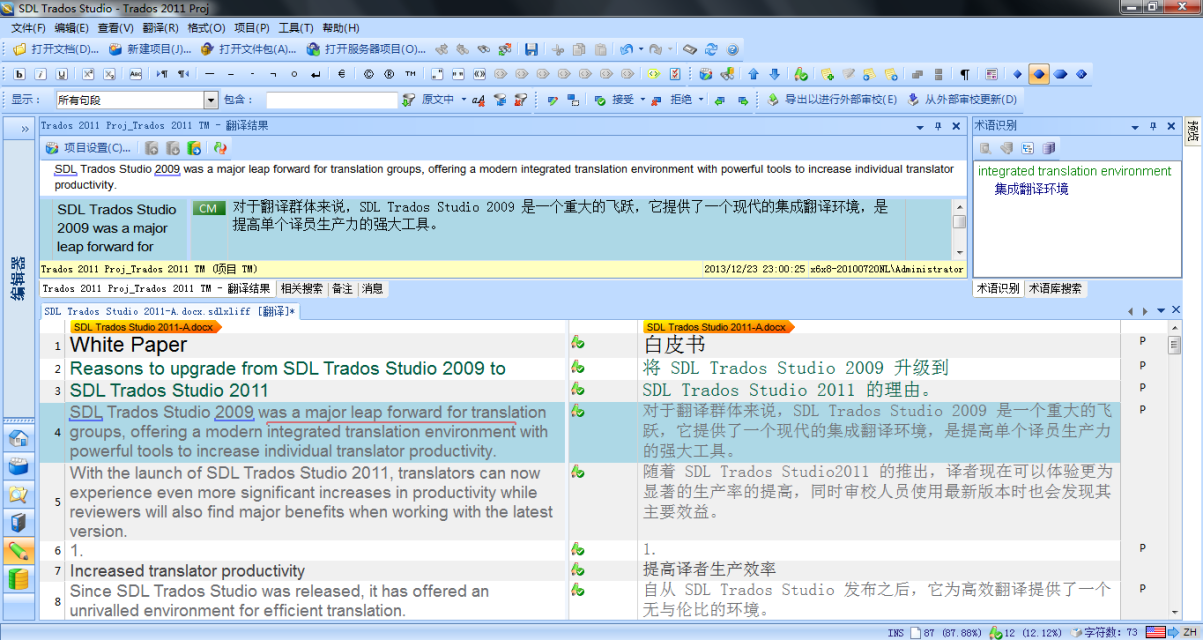
\includegraphics[width=0.98\textwidth]{Figure/Figure_2_7.png}
	\caption{典型的计算机辅助翻译软件界面(Trados)}
	\label{Fig_cat_trados}
\end{figure}

除了翻译记忆功能,计算机辅助翻译系统一般还包括文件格式解析器、完全匹配与模糊匹配、上下文匹配、相关性搜索、断句规则和语料对齐等功能。在人工翻译流程中,计算机辅助翻译的作用可以总结为:复用翻译记忆和术语库等语言资产、控制翻译质量、简化翻译格式、辅助翻译协作、辅助翻译管理等。主流的计算机辅助翻译商业软件有Trados、MemoQ、Wordfast、Déjàv、Memsource、OmegaT、Wordbee等等。典型的计算机辅助翻译软件如图\ref{Fig_cat_trados}所示,限于篇幅,本文不展开论述计算机辅助翻译软件。

\section{人机交互式机器翻译}

在本文中,我们将面向计算机辅助翻译的机器翻译称作人机交互式机器翻译。人机交互式机器翻译通过融合现有的机器翻译和计算机辅助翻译,使之成为生产力工具,最终以提高人工翻译效率为目的。借鉴文献[\cite{Hutchins:1992}],我们对人机交互式机器翻译的定位如图\ref{Fig_automation_degree}所示。在图\ref{Fig_automation_degree}中,从左到右翻译自动化程度越来越低,人机交互式机器翻译和计算机辅助翻译介于机器翻译和人工翻译二者之间,翻译主体是人,机器处理辅助地位。人机交互式机器翻译的自动化程度比计算机辅助翻译高,介于机器翻译与计算机辅助翻译之间。

\begin{figure}[!tb]
	\centering
	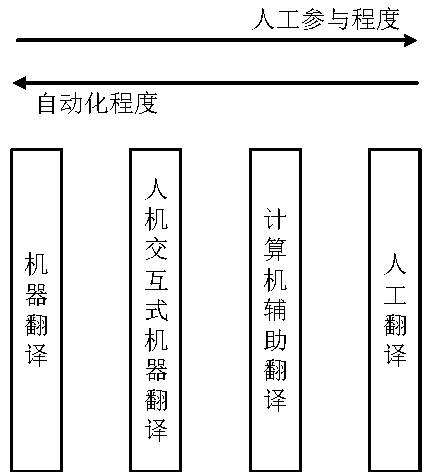
\includegraphics[width=0.6\textwidth]{Figure/Figure_2_8.pdf}
	\caption{翻译自动化程度}
	\label{Fig_automation_degree}
\end{figure}

为了将机器翻译与计算机辅助翻译融合到一起,我们需要回答三方面的问题:(1)什么样的人机交互方式有利于译员提高翻译效率;(2)如何将记忆库和术语库等语言资产与机器翻译挂接起来;(3)如何让译员干预机器翻译系统的自动译文。目前融合机器翻译与计算机辅助翻译的研究还处于萌芽阶段,接下来,我们将介绍已有的相关工作,并提出本文的研究思路。

\subsection{译后编辑}

译后编辑最早由Elizabeth Wagner提出[\cite{Wagner:1985}],简单而言就是通过人工直接修改机器翻译的自动译文来完成翻译。译后编辑是最简单的人机交互方式。Trados等计算机辅助翻译工具通常支持谷歌翻译等API来直接获取机器翻译的自动译文,因此译后编辑是目前最流行的辅助形式。如果机器翻译的自动译文质量较高,人工修改量就比较少,这种方式可以有效提升译员的生产效率[\cite{Car:2011,Koehn:2012,Zhechev:2012}]。但在行业实践中,译后编辑面临诸多现实挑战,有时甚至仅仅是聊胜于无。主要原因在于当前的机器翻译系统对应的译文质量远未达到人工翻译场景的用户期望[\cite{Thicke:2013,Moorkens:2015}]。如果机器翻译的自动译文质量较差,译员不得不为了少打几个字而被迫分析和修改漏洞百出的整句译文,其代价远超过直接翻译。僵化的译文和似是而非的术语翻译使得译员使用机器翻译的热情并不高,而重复纠正相同错误的乏味感和反复修改仍不能满意的挫败感也使用户感到沮丧。针对前述问题,已有相当多的工作尝试解决[\cite{Koehn:2009a,Simard:2013,Green:2014,Denkowski:2014,Wuebker:2015}]。近两年来,神经网络机器翻译(neural machine translation,NMT)发展迅猛[\cite{Zhang:2015,LiXiaoqing,TuZhaopeng:2016,Shen:2016}],译文质量显著提升,同时也带来了新的挑战,如“顺而不信”和翻译结果难以干预等问题。因此,神经网络机器翻译仍需要相当长时间才可能在实践中显著改善译后编辑的人机交互体验。

\subsection{交互式机器翻译}

交互式机器翻译指系统根据用户已翻译的部分译文动态生成后续译文候选供用户参考,最早由Feorge Foster提出[\cite{Foster:2002}]。译员从零开始翻译,因此译员无需修改自动译文,仅在翻译过程中选择可接受的部分即可。该技术指在通过翻译人员与机器翻译引擎之间的交互作用,从而实现人类译员的准确性和机器翻译引擎的高效性。

\begin{figure}[!tb]
	\centering
	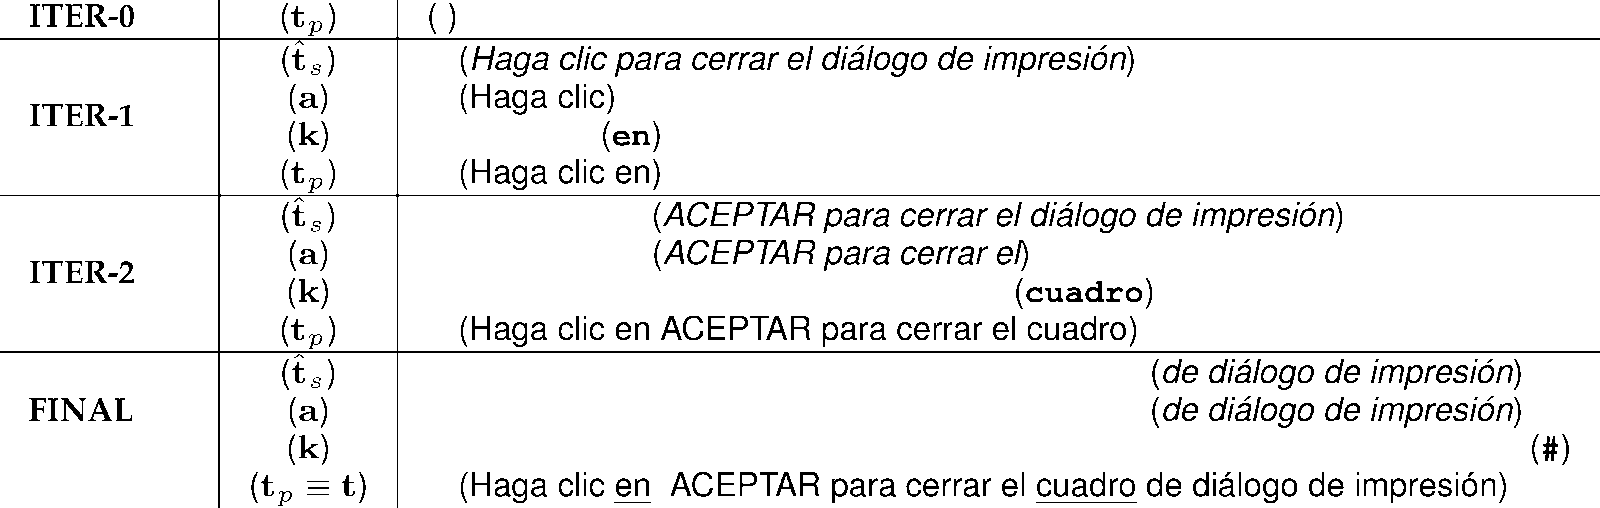
\includegraphics[width=0.98\textwidth]{Figure/Figure_2_9.png}
	\caption{交互式机器翻译}
	\label{Fig_imt_procedure}
\end{figure}

典型的交互式机器翻译如图\ref{Fig_imt_procedure}英译法翻译过程所示[\cite{Barrachina:2009}]。在每一轮人机交互中,初始状态为上一步已确定的法语(目标语言)前缀 ,机器翻译系统根据 生成新的法语后缀 。译员可以根据需要接受 的一部分,如符号 所示。然后,译员继续用键盘输入目标语言词,如符号 所示。直到译员输入译文结束符“\#”完成整个句子的翻译。

与译后编辑相比,交互式机器翻译系统对技术实现有更高的要求:从左至右的强制解码和流畅的实时响应。同时,因为需要译员反复阅读和理解最新的译文部分,这种模式也给用户带来了额外负担。因此,目前流行的在线翻译系统和计算机辅助翻译工具并不支持交互式机器翻译模式。目前的交互式机器翻译系统仍处于原型阶段[\cite{Koehn:2009b,Koehn:2014,Cheng:2016}]。可喜的是,从近期机器翻译技术的发展,尤其是基于神经网络机器翻译的交互式机器翻译[\cite{Knowles:2016}]的进步可以预见,交互式机器翻译有望成为未来人工翻译的候选项之一。

\subsection{术语翻译}

术语广泛存在于具体的领域语料中,如计算机和医学领域。受限于专业背景,术语翻译一直是专业译员面临的首要难题。根据文献[Austermühl, 2014],专业译员在术语翻译上所用的时间多达75\%。可见术语翻译对于人机交互式机器翻译至关重要。

术语翻译主要包含三方面的问题:术语识别、术语翻译知识挖掘和术语翻译知识融合。术语识别是术语翻译知识挖掘和正确翻译的前提,术语翻译知识融合主要解决如何将挖掘到的术语翻译知识与机器翻译解码器进行有机融合的问题。

术语识别是指从文本中自动发现领域术语的过程。它是一项具有重要作用的语言技术,在自然语言处理、机器翻译等应用领域具有重要意义。自动术语识别常用的方法包括基于规则方法和基于统计方法。基于规则方法是根据术语构成模式建立一套规则,选择匹配规则的词语作为领域术语[\cite{Ananiadou:1994,Dagan:1994,Frantzi:1999}]。这种方法的最大缺陷是人工编写的规则不可能覆盖所有的语言学现象,领域依赖性很强。基于统计方法主要应用词频、TF-IDF[\cite{Evans:1995,Martins:2010}]、t-test[\cite{Fahmi:2007,Wermter:2005}]、C-value/NC-value[\cite{Frantzi:1999,Frantzi:2000}]、互信息[\cite{Daille:1996}]、信息熵、log-likelihood[\cite{Cohen:1995,Lefever:2009}]、假设检验或者其它统计特征[\cite{Burkett:2010b,Kozakov:2004,Park:2002,Sclano:2007}],选择特征值符合阈值的词语作为领域术语。但现实中还没有任何一种方法能解决实际中的术语识别问题,与命名实体识别的性能还有很大的差距。基于统计方法不受领域限制,但是对于多词术语和低频术语的识别并不理想,抽取的术语也存在较多噪声。为了增强方法的通用性和实用性,本文关注采用了机器学习技术的术语识别方法(如最大熵模型),即通过对训练集文本特征的学习构造模型来进行术语识别。当前术语识别的性能并没有达到能直接用于术语翻译知识挖掘的水平。其主要原因为如下两点:(1)性能更好的基于机器学习技术的术语识别方法需要高质量的人工标注数据,但目前极度缺乏足量且高质量的术语标注数据;(2)不断有新的术语产生,标注数据的更新速度严重滞后于实际需求。

术语翻译知识广泛存在双语平行句对和单语语料中,尤其是互联网网页中存在海量的术语翻译知识。按照翻译知识的来源划分,现有的术语翻译挖掘方法主要分为三类:(1)从双语平行句对中挖掘[\cite{Fan:2009,LiXiuying:2009}];(2)从可比语料中挖掘[\cite{Fung:1997}];(3)从互联网单语语料中挖掘[\cite{Cao:2007,Ren:2010}]。一般而言,主流的双语术语挖掘流程中,第一步是根据预先定义的模式[\cite{Kupiec:1993}]、统计特征[\cite{Lefever:2009}]或者有监督机器学习[\cite{Fan:2009}]等方法先识别源语言和目标语言术语。术语翻译知识抽取面临的主要挑战是,较差的术语识别性能导致的准确率和召回率都比较低,最后生成的双语术语词典的噪声比较大。如Vintar发现利用统计方法从平行句对抽取出的双语多词术语翻译对可用性比较差,而通过句法模式匹配能抽取出高可用的术语对,而后者又受限于人工标注的语料规模[\cite{Vintar:2001}]。

命名实体有明确的特征和边界信息,而术语的界定相对比较困难,因此难以直接应用命名实体翻译知识的抽取方法。Burkett等人[\cite{Burkett:2010a}] 建立一个多视角学习(multiview learning)目标以强制单语和双语命名实体识别模型结果达成一致,通过未标注的双语语料模拟训练双语识别模型,然后在一个性能比较强的单语命名实体识别模型的基础上,提升另一个性能比较弱的单语命名实体识别模型。但在术语识别问题上,很难训练得到一个性能非常强的单语识别模型,所以很难通过这种方法去提高另一个更弱的术语识别模型。Wang等人[\cite{Wang:2013a}]设计了一种对偶分解算法,在[\cite{Martins:2010,Martins:2011,Riedel:2011}]方法基础上,对命名实体识别和词对齐进行联合解码,并通过实体跨度和实体类型来纠正词对齐错误。对于术语而言,我们很难定义细分类型,仅有术语跨度信息可用,加之缺乏高质量标注语料,因而对偶分解这种方法的效果会大打折扣。

术语翻译知识融合方面,一般是以直接查询双语术语库的方式与机器翻译解码器结合起来。这种融合方法比较简单直接,但缺陷也同样明显。一方面,在术语用词的范围非常广,而术语识别性能又比较低的情况下,简单的字符串匹配会直接导致较多的匹配错误。另一方面,由于双语术语对有明显的长尾效应,存在海量的低频专业术语,直接融合大规模双语术语库的方法会影响机器翻译解码器的正常翻译过程,从而降低最终的机器翻译性能。

\subsection{融合翻译记忆的统计机器翻译}

根据文献[\cite{Kay:1980,Somers:2004}],翻译记忆的核心思想是,如果有了翻译过的相似文档,则可以直接抽取其中相似的部分来辅助翻译。从本质上讲,翻译记忆仅仅是一种辅助翻译的工具,它注重的是对已有翻译的复用,指在减少翻译过程中专业译员的重复劳动。直到最近几年,随着统计机器翻译质量的不断提高,研究人员才开始关注如何结合翻译记忆与统计机器翻译,并由此开展了一系列的探索工作。

翻译记忆与统计机器翻译的融合方法,根据处理的基本单元的不同,我们可以将它们分为两类:(1)以句子为单位的融合方法[\cite{He:2010a,He:2010b}];(2)以匹配片断为单位的融合方法[\cite{Bicici:2008,Simard:2009,Smith:2009,Koehn:2010,Zhechev:2010,He:2011,Wang:2013b,wangkun:2013}]。以句子为单位的融合方法,是以句子为基本单位,从机器翻译输出和翻译记忆系统的参考翻译中,挑选最好的结果,并不修改这些输出结果。以匹配片断为单位的结合方法,则是以匹配片断为基本单位,从翻译记忆系统给出的参考翻译中,抽取匹配片断相关的信息,来指导机器翻译进行解码。

\subsection{在线自适应}

人机交互式机器翻译系统在线自适应是统计机器翻译的一项核心任务,它从用户当前上下文或者已提交的最新完成的翻译句子中发掘新的翻译知识,并实时更新模型,最终得到在当前场景中质量更好的自动译文。因此,如果能利用人工翻译过程使人机交互式机器翻译系统完成在线自适应(online adaptation),能显著提升自动译文的质量,进而增强机器翻译的可用性。需要注意的是,在本文中,在线自适应,包括但不限于增长式学习、在线学习和其它各种能实时更新系统参数的方法。

目前已有的人机交互式机器翻译的在线自适应方法,根据自适应对象的不同,我们可以将它们大致分为四类:(1)词对齐模型的自适应[\cite{ZhaoBing:2002,Hardt:2002,Mccarley:2011,Blain:2012,Farajian:2014}];(2)增加新的翻译规则到翻译模型中[\cite{Nepveu:2004,Hardt:2002,Ortiz-Martinez:2010,Simard:2013,Denkowski:2014,Bertoldi:2014}];(3)语言模型的自适应[\cite{Bertoldi:2014,Denkowski:2014}];(4)参数在线学习[\cite{Bertoldi:2014,Denkowski:2014}]。其中,词对齐模型的自适应是抽取新的翻译规则的前提条件,主要需要解决未登录词和低频词的对齐问题。增加新的翻译规则到翻译模型中,最直接同时最简单的方法是[\cite{Bertoldi:2014}]提出的内部缓存和外部缓存。内部缓存,即常规翻译模型之外的一个小型翻译模型,类似于计算机操作系统的缓存,新的翻译规则不断被插入,然后根据在缓存中的时间长短对翻译规则进行排序,新进的翻译规则得分最高。外部缓存,指翻译一句时将外部抽取的翻译规则加入到已检索到的常规翻译规则中。通过外部缓存可以直接干预术语和命名实体的机器翻译结果,通过内部缓存可以使机器翻译快速适应当前的上下文。现有的在线自适应方法主要面临新旧知识的调和以及算法计算复杂度的挑战。通常而言,简单直接的内部缓存和外部缓存在短期内立竿见影,但随着数据的增加,对性能的改善越来越不明显。由于语言模型的自适应和参数在线学习不是本文的关注点,所以不再赘述。

综上所述,人机交互式机器翻译正处于走向实用化的关键时期,在未来仍然主要面对三方面的问题:用户如何更高效地使用机器翻译;机器翻译如何利用已有的外部资源提高自动译文质量以减少用户的重复劳动;机器翻译如何根据用户上下文进行自适应完成模型和参数的自动更新。这三个问题也是本文致力于解决的问题。

\section{本文的研究思路}

从最初基于词的翻译模型,到现在神经网络机器翻译,机器翻译研究者们一方面通过不懈地研究和探索,极大地改善了机器翻译的质量。另一方面,研究者还提出了一系列人机交互式机器翻译方法,试图提供良好的人机交互,最大限度复用术语和翻译记忆等语言资产,在线自适应以完成模型和参数的自动更新。

译后编辑在人机交互式机器翻译的交互方式上取得了较大的成功,也是目前专业译员利用机器翻译的主流方式。但由于过度依赖机器翻译的译文质量,译后编辑还存在许多问题。因此,本文首先从人机交互方式入手,尝试提出新的与机器翻译交互的方式。本文将提出融合统计机器翻译知识的中文输入方法,通过充分利用统计机器翻译知识,使机器翻译在无法提供高质量自动译文的情况下,也能极大地提高译员的人工翻译效率。第三章将介绍我们提出的中文输入方法。

虽然目前已经有各种各样的改进术语翻译质量的方法,但大多数方法要么依赖高质量的人工标注数据训练的术语识别分类器,要么受制于从互联网语料抽取的带有很多噪声的术语翻译词典。由于术语翻译问题本身的艰巨性,目前主流的机器翻译系统往往不专门考虑术语翻译问题。为此本文提出了融合术语识别边界的术语翻译方法,从多种来源挖掘术语翻译知识,并有效地利用挖掘到的术语翻译知识。该方法以低质量的自然标注数据为起点,从双语平行句对和广泛存在的网络单语语料中挖掘术语翻译知识,并尝试通过融合术语边界信息的统计翻译术语解码方法使统计机器翻译解码器更有效地利用已挖掘到的术语翻译知识。第四章将介绍我们提出的术语翻译方法。

不仅人机交互方式和术语翻译比较重要,而且机器翻译的在线自适应问题也是人机交互式机器翻译不可忽视的重要问题。因为重复纠正相同错误的乏味感让使用机器翻译的专业译员感到沮丧,而这会直接影响到译员对机器翻译系统的接纳程度。基于此,我们探索基于随机森林的统计翻译模型在线学习方法。第五章将介绍我们对基于随机森的机器翻译翻译模型的探索。
最后,我们设计和实现了融合机器翻译和计算机辅助翻译的人机交互式机器翻译系统,并总结了开发过程中遇到的关键问题和应对策略。第六章将介绍人机交互式机器翻译系统的设计和实现。

\section{本章小结}

本章对现有的主流机器翻译方法和人机交互式机器翻译方法进行了简要的介绍。主流机器翻译方法包括基于词的翻译模型、基于短语的模型、基于句法的模型和神经网络翻译方法。人机交互式机器翻译包括人机交互方式、术语和翻译记忆等语言资产复用方法和机器翻译的在线自适应方法。本章还分析了目前机器翻译和人机交互式机器翻译方法在人工翻译场景中存在的问题,并简要说明了本文的解决方法,同时引出了本文对于人机交互式机器翻译方法的研究思路。
